% Options for packages loaded elsewhere
\PassOptionsToPackage{unicode}{hyperref}
\PassOptionsToPackage{hyphens}{url}
%
\documentclass[
]{article}
\usepackage{lmodern}
\usepackage{amssymb,amsmath}
\usepackage{ifxetex,ifluatex}
\ifnum 0\ifxetex 1\fi\ifluatex 1\fi=0 % if pdftex
  \usepackage[T1]{fontenc}
  \usepackage[utf8]{inputenc}
  \usepackage{textcomp} % provide euro and other symbols
\else % if luatex or xetex
  \usepackage{unicode-math}
  \defaultfontfeatures{Scale=MatchLowercase}
  \defaultfontfeatures[\rmfamily]{Ligatures=TeX,Scale=1}
\fi
% Use upquote if available, for straight quotes in verbatim environments
\IfFileExists{upquote.sty}{\usepackage{upquote}}{}
\IfFileExists{microtype.sty}{% use microtype if available
  \usepackage[]{microtype}
  \UseMicrotypeSet[protrusion]{basicmath} % disable protrusion for tt fonts
}{}
\makeatletter
\@ifundefined{KOMAClassName}{% if non-KOMA class
  \IfFileExists{parskip.sty}{%
    \usepackage{parskip}
  }{% else
    \setlength{\parindent}{0pt}
    \setlength{\parskip}{6pt plus 2pt minus 1pt}}
}{% if KOMA class
  \KOMAoptions{parskip=half}}
\makeatother
\usepackage{xcolor}
\IfFileExists{xurl.sty}{\usepackage{xurl}}{} % add URL line breaks if available
\IfFileExists{bookmark.sty}{\usepackage{bookmark}}{\usepackage{hyperref}}
\hypersetup{
  hidelinks,
  pdfcreator={LaTeX via pandoc}}
\urlstyle{same} % disable monospaced font for URLs
\usepackage[margin=1in]{geometry}
\usepackage{graphicx,grffile}
\makeatletter
\def\maxwidth{\ifdim\Gin@nat@width>\linewidth\linewidth\else\Gin@nat@width\fi}
\def\maxheight{\ifdim\Gin@nat@height>\textheight\textheight\else\Gin@nat@height\fi}
\makeatother
% Scale images if necessary, so that they will not overflow the page
% margins by default, and it is still possible to overwrite the defaults
% using explicit options in \includegraphics[width, height, ...]{}
\setkeys{Gin}{width=\maxwidth,height=\maxheight,keepaspectratio}
% Set default figure placement to htbp
\makeatletter
\def\fps@figure{htbp}
\makeatother
\setlength{\emergencystretch}{3em} % prevent overfull lines
\providecommand{\tightlist}{%
  \setlength{\itemsep}{0pt}\setlength{\parskip}{0pt}}
\setcounter{secnumdepth}{-\maxdimen} % remove section numbering

\author{}
\date{\vspace{-2.5em}}

\begin{document}

\hypertarget{MethodsChapter}{%
\section{LRP ESTIMATION METHODS}\label{MethodsChapter}}

In this section, we provide an overview of methods used to develop LRPs
for our three case studies. Detailed methods specific to each case study
are provided in Sections @ref(IFCChapter) (Interior Fraser Coho),
@ref(WCVIchinookChapter) (West Coast Vancouver Island Chinook), and
@ref(ISCchumChapter) (Inner South Coast Chum, excluding Fraser). Links
to GitHub repositories with the data and analysis code used for all
three case studies are in Appendix @ref(app:github-appendix). An
overview of the approaches applied to each of the three case studies are
provided in Table @ref(tab:lrpapproaches).

~ ~

\renewcommand*{\arraystretch}{1.4}
\begin{table}[!htbp]
\setlength\heavyrulewidth{0.25ex}
\centering
\footnotesize   
\caption{Overview of CU assessment methods applied for each case study (a) and approaches used to estimate LRPs (b) }
\begin{tabular}{p{3.2cm} p{3.2cm} p{2.4cm} p{2.4cm} p{2.4cm}}
\multicolumn{5}{l}{(a) CU-level assessments }\\
\toprule
\multicolumn{2}{l}{} & Interior Fraser River Coho & WCVI Chinook & Inside South Coast Chum \\
\toprule
\multicolumn{2}{l}{\parbox{5.8cm}{Multidimensional approach used in the Salmon Scanner}}& Yes (only for proportional LRPs) &   Yes (only for proportional LRPs)  &  Yes (only for proportional LRPs)\\
\midrule
\multirow{3}{*}{\parbox{3.2cm}{Single metric approaches: spawner abundances relative to benchmark}} & Spawner-recruitment benchmark & Yes & - & Attempted, estimates unreliable\\
\cline{2-5}
& Habitat-based benchmark & - & Yes & -\\
\cline{2-5}
& Percentile benchmark & - & - & Yes\\
\cline{1-5}
\multicolumn{2}{l}{Single metric approaches: distribution} & Yes & - & - \\
\bottomrule
\multicolumn{5}{l}{ }\\
\multicolumn{5}{l}{(b) LRPs }\\
\toprule
\multicolumn{2}{l}{} & Interior Fraser River Coho & WCVI Chinook & Inside South Coast Chum \\
\toprule
\multicolumn{2}{l}{Proportional LRP} &  Yes &   Yes &   Yes\\
\midrule
\multirow{2}{*}{\parbox{3.2cm}{Aggregate abundance LRPs}} & Logistic regression LRP & Yes & Attempted, data insufficient &  Attempted, estimates unreliable \\ 
\cline{2-5}
 & Projection LRP & Yes  & Yes &  - \\
\bottomrule
\end{tabular}
(\#tab:lrpapproaches)
\end{table}

~ ~ ~

\hypertarget{overview}{%
\subsection{OVERVIEW}\label{overview}}

We consider two types of LRPs based on two different metrics:

\begin{enumerate}
\def\labelenumi{\arabic{enumi})}
\item
  Proportional LRPs use a proportion as the metric upon which LRPs are
  based. Specifically, they use the proportion of CUs within an SMU that
  are above the Red WSP status zone. We assume that in order for an SMU
  to remain above its proportional LRP, 100\% of CUs must have status
  estimates above Red (i.e., either Amber or Green).
\item
  Aggregate abundance LRPs use the total SMU-level spawning abundance as
  the metric upon which LRPs are based. Two methods of developing
  aggregate abundance LRPs are applied: (i) Logistic Regression LRPs and
  (ii) Projection LRPs.
\end{enumerate}

We propose that proportional LRPs are more appropriate for Pacific
salmon SMUs because they more directly align with DFO's WSP objectives
of maintaining salmon biodiversity; however, aggregate abundance LRP
methods may be added to meet specific fisheries management requirements.

We implement proportional LRPs using approaches developed to assess CU
status under DFO's WSP {[}@dfoCanadaPolicyConservation2005;
@holtIndicatorsStatusBenchmarks2009{]} and implemented for a subset of
priority CUs {[}@dfoWildSalmonPolicy2015;
@dfoIntegratedBiologicalStatus2016; @grant2017FraserSockeye2020{]}.
These approaches use multiple metrics to evaluate status including
trends in abundance and abundance metrics, and an expert-driven
integration approach to combine statuses across metrics into a single
status for each CU. In our case study applications, we apply the
recently developed Pacific Salmon Status Scanner tool (hereafter
referred to as the `Salmon Scanner'; Pestal et al., in prep\footnote{Pestal,
  G., MacDonald, B, Grant, S, and Holt, C., in prep. Rapid Status
  Approximations from Integrated Expert Assessments Under Canada's Wild
  Salmon Policy. Can. Tech. Rep.~Fish. Aquat. Sci.}) as a way to rapidly
approximate more detailed WSP status assessments. The Salmon Scanner
allows us to rapidly generate up-to-date estimates of integrated CU
status for all of our case study applications, and is recommended as an
approach for defining LRPs in our companion working paper (Holt et al.,
in review).

When developing candidate aggregate abundance LRPs, we aim to maintain
consistency with the WSP by defining LRPs as aggregate abundance levels
that have a high probability of all CUs being above their Red status
zone. For these LRPs, estimates of CU status are approximated based on a
comparison of spawning abundance to a single lower benchmark for each
CU. Exceptions are described in the application to case studies.

We also maintain consistency with the WSP by only including spawning
streams without significant enhancement when evaluating CU and SMU
status. We use the Proportionate Natural Influence metric, PNI,as a
basis for defining `significant enhancement'. PNI is a metric designed
to estimate the relative strength of the hatchery and natural selective
pressures resulting from gene flow between the two environments, and is
used as a basis for determining genetic risk of hatcheries on natural
populations. Values less than 0.5 indicate populations where most fish
are hatchery origin {[}classified as integrated-hatchery populations;
@withlerGeneticallyBasedTargets2018{]}. We defined `significantly
enhanced' populations as those with PNI values \(<\) 0.5 and excluded
them from case study analyses.

Systems with levels of PNI \(\geqslant\) 0.5 can still have hatchery
influences; however, dynamics are predominately natural origin. Where
time-series of the proportion of hatchery marked fish on the spawning
grounds are available (e.g., Interior Fraser Coho case study), these
proportions are used to inform assessments in two ways: first to develop
time-series of natural-origin recruitment for benchmark estimation based
on stock-recruitment relationships and second to develop time series of
natural-origin spawners for status assessment against benchmarks. When
reliable time-series of the proportion of hatchery influence are not
available (WCVI Chinook), total spawners are used for LRP analyses
provided that the threshold of assumed PNI \(\geqslant\) 0.5 has been
met.

More detailed descriptions of LRP estimation methods are provided in the
following sections, while guidance on when and how proportional and
aggregate abundance LRPs should be applied is provided in Holt et
al.~(in review). We recommend that users consult Holt et al.~(in review)
before applying any of the methods described in this case study paper.

\hypertarget{proportional-lrps}{%
\subsection{PROPORTIONAL LRPS}\label{proportional-lrps}}

A proportional LRP was set as 100\% of CUs above their red Red status
zone. The LRP therefore acts as a trigger that is breached when one or
more CUs in an SMU is assessed as having Red status. Rationale for this
choice of 100\% of CUs required to be above Red status is described in
Holt et al.~(in review).

We compare three different methods of assessing CU status when using
proportional LRPs: (i) the proportion of CUs with a recent WSP status
assessment above the Red zone (e.g., @grant2017FraserSockeye2020), (ii)
the proportion of CUs with a recent Salmon Scanner status assessment
above Red (see below for more details), and (iii) the proportion of CUs
with status estimated to be below a single CU lower benchmark (e.g.,
S\textsubscript{gen}, percentile-based benchmarks, etc.). We recommend
methods (i) and (ii) for CU assessments, and provide method (iii) for
comparison purposes.

When assessing CU status relative to a single abundance-based lower
benchmark in approach (iii), we compare generational mean spawner
abundances to the benchmark, as described in Holt et al.~(In review).

\hypertarget{rapidToolMethods}{%
\subsubsection{MULTIDIMENSIONAL APPROACH TO CU STATUS ASSESSMENTS WITHIN
THE PACIFIC SALMON STATUS SCANNER}\label{rapidToolMethods}}

The Pacific Salmon Status Scanner (the Salmon Scanner) estimates
statuses for individual WSP metrics and also integrates the statuses on
multiple metrics into a single status estimate (e.g., Red, Amber, Green;
Pestal et al., in prep). By automating this process, the Salmon Scanner
supports implementation of Canada's WSP by rapidly approximating the
more detailed, comprehensive WSP status assessment process. The Salmon
Scanner's approach can be implemented annually and for a broader range
of CUs, given it is less time and labour intensive that full WSP status
assessments. The Salmon Scanner was developed using Classification and
Regression Tree (CART) analyses, and expert judgement gained from
integrated status assessment processes, to create algorithms that
approximate the integrated status assessment results.

Data inputs and outcomes from previous WSP assessment processes were
used in the Salmon Scanners analyses: Fraser River Sockeye, Interior
Fraser Coho, and Southern BC Chinook {[}@dfoWildSalmonPolicy2015;
@dfoIntegratedBiologicalStatus2016; @dfo2017FraserSockeye2018;
@grant2017FraserSockeye2020{]}. Briefly, the Salmon Scanner uses a
decision tree to estimate CU status based on data type, quality,
abundance, and trends (e.g., Figure @ref(fig:decision-tree)). The
decision tree algorithm was verified with data and local expertise
(Pestal et al.~in prep). As with other methods, an expert review of
rapid status results for each CU is intended to be incorporated into the
application of this tool (S. Grant, pers. comm.). When using this method
in the case study, we took the outputs of the algorithms at face value
and did not confirm them based on expert opinion. In practice, results
from the Salmon Scanner will be validated against local expertise when
implemented annually (S. Grant, pers. comm.).

For absolute or relative abundance metrics, the Salmon Scanner uses the
most recent generational mean spawner abundance (calculated as a running
geometric mean) to compare to benchmarks, including absolute abundance
thresholds (e.g., 1500 spawners), abundance-based lower benchmarks
(e.g., S\textsubscript{gen} or percentile), and abundance-based upper
benchmarks (e.g., 0.8S\textsubscript{MSY} or percentiles). Generational
mean spawner abundances as also used when calculating trends in spawner
abundances over time (Pestal et al., in prep.)

\newpage
\begin{landscape}

```
## Linking to librsvg 2.48.8
```

\begin{figure}

{\centering 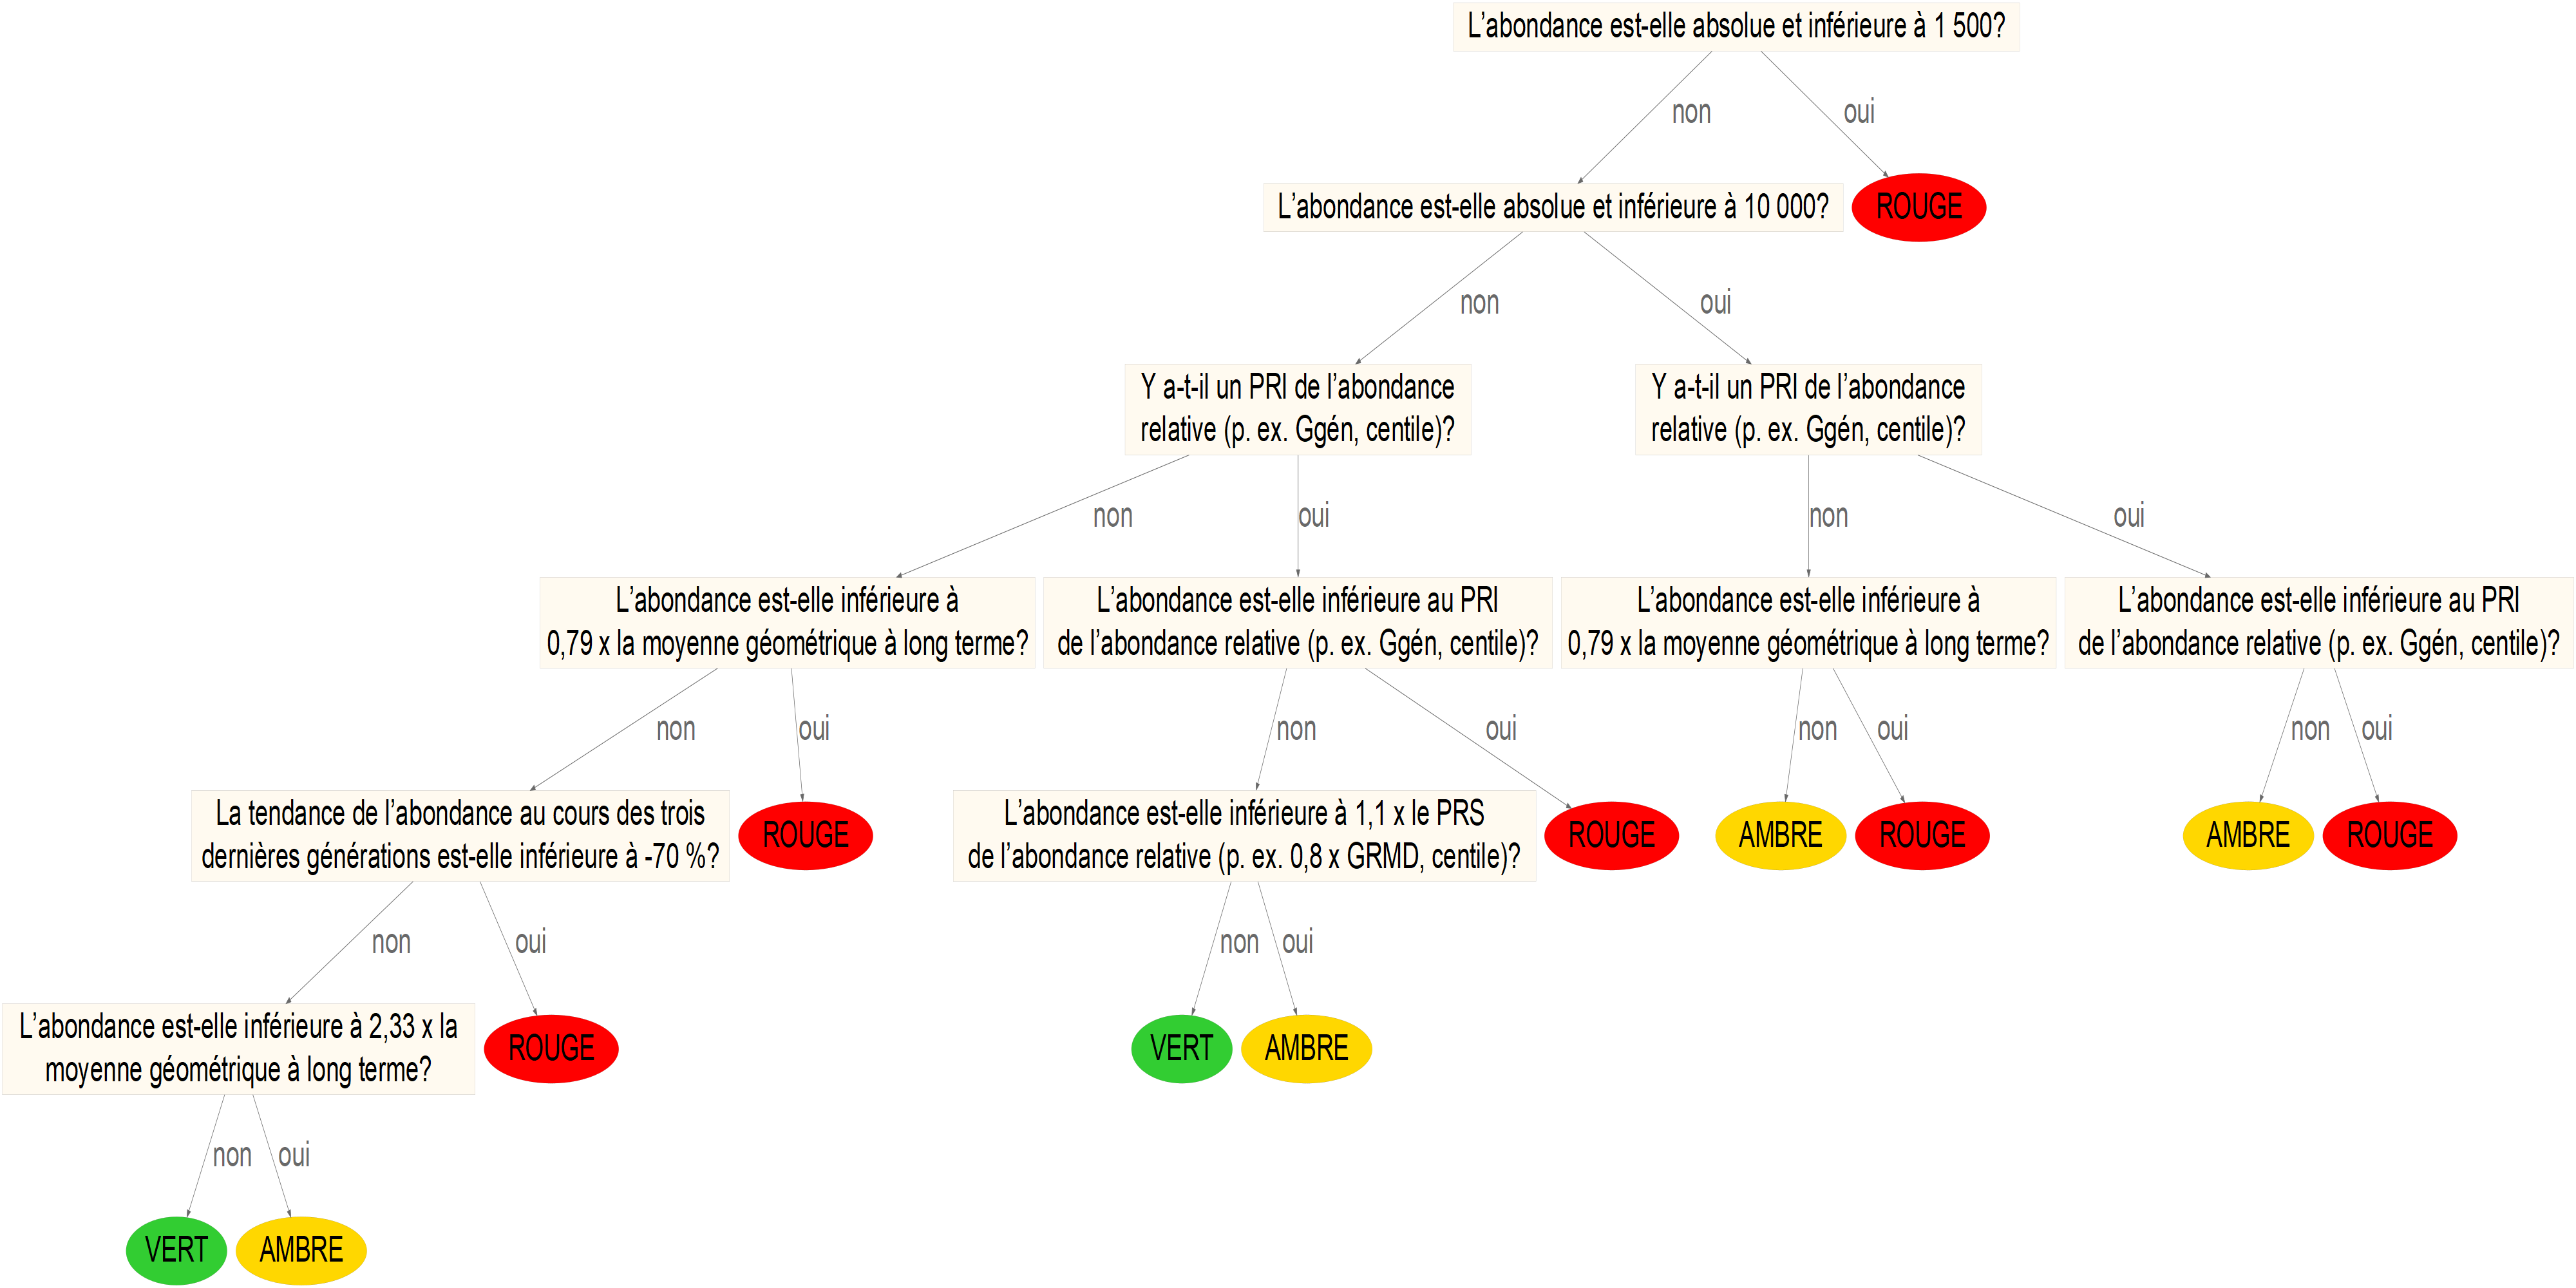
\includegraphics[width=1\linewidth]{figure/decision_tree} 

}

\caption{Decision tree (also referred to as the multidimensional algorithm) used in the Pacific Salmon Status Scanner to assess status of Conservation Units based on multiple metrics under the Wild Salmon Policy (Pestal et al. in prep.)}\label{fig:decision-tree}
\end{figure}
\end{landscape}

\hypertarget{aggAbundMethods}{%
\subsection{AGGREGATE ABUNDANCE LRPS}\label{aggAbundMethods}}

Aggregate abundance LRPs are based on the assumption that there is a
predictable relationship between SMU-level abundance and the probability
that all CUs will be above Red status. When estimating aggregate
abundance LRPs, status relative to a single lower benchmark (LBM) is
used a proxy for status above the Red zone. Aggregate abundance LRPs are
then estimated by using the predicted relationship to find the SMU-level
abundance at which there is a prescribed probability that 100\% of CUs
(the same proportion that was used for proportional LRPs) will be above
the LBM.

The above definition of aggregate abundance LRPs requires a decision to
be made about the required probability that 100\% of CUs will be above
their LBMs. We consider four alternative probability levels for our case
studies that represent a range of calibrated probability categories
developed by the Intergovernmental Panel on Climate Change
{[}@frameGuidanceNoteLead2010{]}: 50\%, 66\%, 90\%, and 99\%. The 50\%
value represents the mid-point of the ``About as likely as not''
category (33 - 66\%), indicating that there is an equal probability that
all CUs will be above their LBMs as there is that they will not. The
66\% values represents the lower end of the ``Likely'' category (i.e.,
it is ``Likely'' that all CUs will be above their LBMs), the 90\% value
represents the lower end of the ``Very Likely'' category, and the 99\%
value represents the ``Virtually Certain'' category. A discussion of
considerations for selecting the appropriate probability threshold when
calculating abundance LRPs is included in (Holt et al.~in review).

We consider two types of aggregate abundance LRPs in our case studies:
logistic regression LRPs and projection LRPs. These two methods differ
in the approach taken to estimate the underlying relationship between
SMU-level aggregate abundance and the probability that all CUs will be
above their LBMs. Logistic regression LRPs are estimated by fitting
statistical models to historical data to estimate this relationship. In
this case, LRPs are based on previously observed covariation in CU
status, and thus implicitly assume the past is a reasonable
approximation of the future. In comparison, projection LRPs use
historical data as a basis for quantifying population dynamics, and then
project population dynamics using stochastic simulations to identify an
equilibrium state. Simulation outputs are then used to characterize the
underlying relationship between aggregate abundance and the probability
that all CUs will be above their LBMs.

The projection LRP approach allows uncertainty in current (or future)
processes that might affect estimation of the LRP to be accounted for
through alternative scenarios. For example, if there is evidence of
recent changes in covariation among CUs, possibly due to a subset of CUs
experiencing reduced productivity, this hypothesis can be modelled in
projections. In comparison, logistic regression LRPs are limited to
using historically observed data, which may not include enough
observations of the new and emerging covaration structure.

For both logistic regression and projection LRPs, we characterize annual
CU status using a single metric, spawner abundances relative to a LBM,
instead of using the status from the multidimensional algorithm within
the Salmon Scanner tool. While in theory, estimates of CU status from
the multidimensional approach could be used for logistic regression
LRPs, we found little evidence of a statistical relationship between CU
statuses from the Scanner and aggregate spawner abundances for the one
case study where we considered this approach, Interior Fraser Coho. We
provide further discussion of this result within the Interior Fraser
Coho case study section of this paper. In addition, projection LRPs are
derived from equilibrium conditions identified from projections that do
not incorporate temporal dynamics required for assessment of trends in
the multidimensional approach. While estimates of CU status relative to
a single LBM such as S\textsubscript{gen} is a readily available output
from the Salmon Scanner tool, we calculated these metrics external to
the tool for our case studies.

When assessing CU status for the purpose of estimating aggregate
abundance LRPs, we used unsmoothed annual spawner abundances instead of
generational averages. This approach was based on preliminary analyses
of the logistic regression method that showed using unsmoothed spawner
abundances improved the spread in the data used to establish a
relationship between CU status and aggregate spawning abundance.
Furthermore, using generational means in the logistic regression
approach led to considerable autocorrelation in the aggregate abundance
time series, violating assumptions of the logistic regression.

However, when assessing SMU status, we used generational running
averages (geometric average) of aggregate spawner abundances. This
approach reduced variability in annual decisions about whether an LRP
had been breached arising from variability in cohorts within a
generation. The decision to use generational averages of aggregate
spawner abundances when determining whether an LRP is breached is
consistent with the approach used for proportional LRPs. In both cases,
the underlying metric being used to determine SMU status (either
aggregate abundance or CU-level status of component CUs for the
proportional approach) is based on generational-averaged values in order
to reduce annual variability in status.

\hypertarget{logisticMethods}{%
\subsubsection{Logistic regression LRPs}\label{logisticMethods}}

Logistic regression LRPs are derived from an empirically estimated
relationship between CU-level status and aggregate SMU abundance. Using
this approach, the LRP represents the aggregate abundance level that has
historically been associated with a given probability of 100\% of CUs
having status above a selected LBM. For each year of observed data,
CU-level status is quantified as a Bernoulli variable: 1 (success) = all
CUs have estimated status greater than their LBM and 0 (failure) = all
CUs do not have status \textgreater{} LBM. A logistic regression is then
fit to these outcomes to predict the probability that all CUs will have
status \textgreater{} LBM as a function of aggregate SMU spawner
abundance using the logistic regression equation:

\begin{equation}
  \log(\frac{p}{1-p}) = B_0 + B_1 \sum_{i}^{i=nCUs} S_{i,t}
   (\#eq:logistic)
\end{equation}

where, \(p\) is probability, \(B_0\) and \(B_1\) are estimated logistic
regression parameters and \(S_{i,t}\) is spawner abundance to CU \(i\)
in year \(t\). Equation @ref(eq:logistic) is then re-arranged to
calculate the LRP as the aggregate spawner abundance associated with the
pre-specified probability threshold of \(p^*\),

\begin{equation}
  LRP = \frac{log(\frac{p^*}{1-p^*}) - B_0}{B_1}
  (\#eq:logisticLRP)
\end{equation}

An example logistic regression fit is shown in Figure
@ref(fig:example-logisticFit). We show the estimation of LRPs based on
this fit for four possible probability thresholds: \(p^*\) = 0.5, 0.66,
0.90, and 0.99. For each \(p^*\) level, LRP estimates represent the
aggregate abundance that is associated with that probability of all CUs
having status greater than their LBM. LRPs were calculated from
parameters of the logistic regression model (Eqn. @ref(eq:logisticLRP)),
with uncertainty in the LRP quantified based on a 95\% confidence
interval on the maximum likelihood estimate, MLE.

\begin{figure}

{\centering 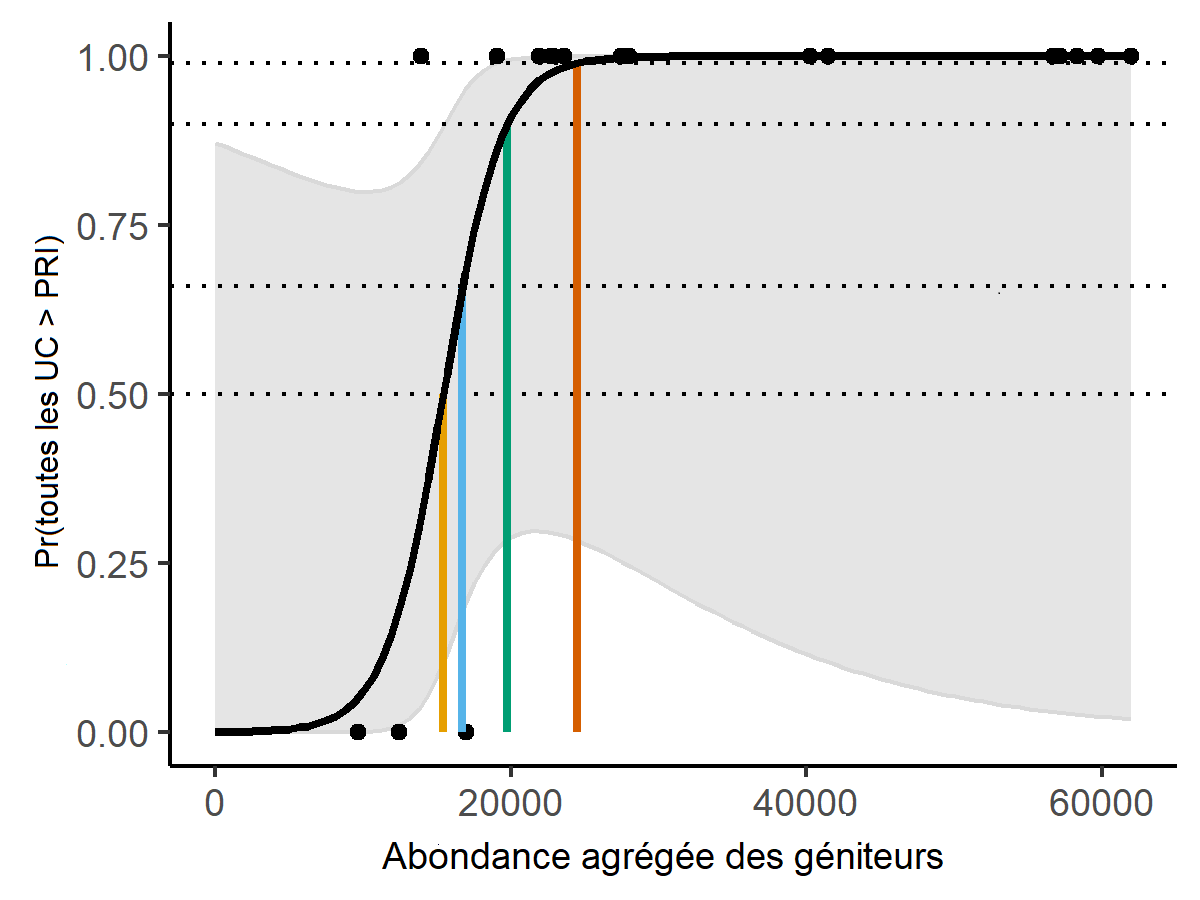
\includegraphics[width=0.6\linewidth]{figure/methods-Example-LogisticLRP} 

}

\caption{Logistic regression fit to annual Bernoulli data to predict the probability of all CUs being above their lower benchmark (LBM) as a function of aggregate SMU abundance. Each black dot represent a year in the observed time series as a Bernoulli indicator showing whether the requirement of all CUs above their LBM was met (success = 1) or not (failure = 0) as a function of aggregate spawning abundance to the SMU. The black solid line is the maximum likelihood model fit to indicator data, and the grey shaded region shows the 95\% confidence interval around the fit model. Coloured lines illustrate aggregate abundance LRPs for 4 different probability thresholds: p* = 0.5 (yellow), 0.66 (blue), 0.90 (green), and 0.99 (orange) probability that all CUs > LBM. Horizontal dotted lines intersect the y-axis at each probability threshold, while the solid vertical lines show the corresponding aggregate escapement that will represent the LRP.}\label{fig:example-logisticFit}
\end{figure}

~

We initially considered an alternative approach to logistic regression
in which the LRP represents the aggregate abundance that has
historically been associated with a pre-specified proportion of CUs
being above their lower benchmark. Using this approach, CU-level status
was quantified as the number or CUs with status \textgreater{} LBM for
each year of observed data. A logistic regression was then fit to
predict the proportion of CUs with status \textgreater{} LBM as a
function of aggregate spawner abundance to the SMU (i.e., abundance from
nCUs combined). We do not present this method for our case studies,
however, due to inherent limitations when the required proportion of CUs
above their lower benchmarks is 100\%. Equation @ref(eq:logisticLRP)
cannot be solved directly for a threshold proportion of \(p^*\) = 100\%,
and LRP estimates were highly sensitive to the choice of \(p^*\) value
used as a proxy. Using \(p^*\) = 99\% vs.~\(p^*\) = 99.9\% vs.~\(p^*\) =
99.99\% gave very different LRP estimates.

The logistic regression model was implemented in TMB
{[}@kristensenTMBAutomaticDifferentiation2016{]}. The model was
statistically integrated, which means that both the CU-specific lower
benchmarks (S\textsubscript{gen}) and the SMU logistic regression
parameters were estimated within the same statistical model. The
integrated approach allowed for the propagation of uncertainty in
parameter estimates from the CU level to the SMU level, resulting in
uncertainty intervals that better capture uncertainty in benchmarks as
well as the logistic model fit.

\hypertarget{logistic-regression-model-diagnostics}{%
\subparagraph{Logistic Regression Model
Diagnostics}\label{logistic-regression-model-diagnostics}}

There are several assumptions associated with logistic regression, three
of which are relevant for our application to LRPs and are listed below.
Model diagnostics were applied to evaluate the extent to which those
assumptions were met, as well as statistical significance of model
coefficients, goodness-of-fit, and classification accuracy of LRPs
developed from the logistic regression. The three assumptions are as
follows:

\begin{enumerate}
\def\labelenumi{\arabic{enumi}.}
\item
  The relationship between aggregate abundance and log-odds (the
  logarithm of the odds of all CUs being above their lower benchmark) is
  linear.
\item
  The observations are independent of each other (i.e., residuals are
  not autocorrelated).
\item
  There are no influential outliers.
\end{enumerate}

~

\textbf{Evaluating assumption of linearity (Assumption 1)}

A Box-Tidwell test was used to evaluate linearity by assessing the
significance of an additional interaction term in the logistic
regression,

\begin{equation}
  \log(\frac{p}{1-p}) = B_0 + B_1 \sum_{i}^{i=nCUs} S_{i,t} + B_2 \sum_{i}^{i=nCUs} S_{i,t} \times \log (\sum_{i}^{i=nCUs} S_{i,t})
   (\#eq:BoxTidwelllogistic)
\end{equation}

A significant interaction term \(B_2\), indicates a non-linear
relationship between aggregate abundance and log-odds, violating this
assumption {[}@foxAppliedRegressionAnalysis2016{]}.

~

\textbf{Evaluating independence (Assumption 2)}

Deviance residuals, \(d\), were estimated for each year,

\begin{equation}
   d = \pm \sqrt { -2 ( y \log(\frac{\mu}{y}) + (1-y)\log(\frac{1-\mu}{1-y}) ) }
   (\#eq:DevianceResid)
\end{equation}

where \(\mu\) is the predicted probability of all CUs being above their
lower benchmark and \(y\) is the observation (1 or 0, indicating all CUs
above Red or not, respectively), in a given year
{[}@foxAppliedRegressionAnalysis2016{]}. Equation @ref(eq:DevianceResid)
reduces to {[}@ahmadDiagnosticResidualOutliers2011{]}:

\begin{align}
d = 
\begin{cases}
  - \sqrt { -2 \log(1-\mu) } & \text{, if } y = 0 \\
  \sqrt { -2 \log(\mu)  }  &\text{, if } y = 1
\end{cases}
  (\#eq:DevianceResidy)
\end{align}

The magnitude of lag-1 autocorrelation was then estimated among deviance
residuals and evaluated for statistical significance.

~

\textbf{Evaluating outliers (Assumption 3)}

We recommend identifying influential outliers using leverage statistics
where possible. For our case studies, we identified outliers independent
of their influence because the software used to estimate model
parameters (TMB) does not provide the hat-matrix required to assess
influence of individual points. Instead, we focused on identifying
outliers based on the general rule of thumb that deviance residuals
greater than 2 are considered to be outliers because 95\% of the
distribution is expected to be within 2 standard deviations of the mean.
Further work to identify influential outliers is recommended when other
statistical model fitting tools are used.

~

\textbf{Statistical significance of model coefficients}

Statistical significance of coefficients was evaluated using the Wald
test statistic, calculated from the ratio of the \(B_1\) model
coefficient to the standard error of that coefficient, which is assumed
to be normally distributed. Test statistics and significance were
estimated within TMB {[}@kristensenTMBAutomaticDifferentiation2016{]}.

~

\textbf{Goodness-of-fit}

The goodness-of-fit was evaluated by comparing the ratio of residual
deviance to null deviance, similar to a likelihood ratio. This ratio is
assumed to follow a Chi-square distribution with 1 degree of freedom
derived from the difference in the number of parameters between full and
null models. P-values \textless0.05 indicate significant lack of fit
{[}@foxAppliedRegressionAnalysis2016{]}.

In addition, the pseudo-\(R^2\) was calculated to indicate the ratio of
the model fit to the null model without an independent variable
{[}@dobsonIntroductionGeneralizedLinear2018{]},

\begin{equation}
   \text{pseudo-}R^2 =  1- \frac{\sum_{t}^{t=nYears} d}{\sum_{t}^{t=nYears} d_0} 
   (\#eq:psuedoR2)
\end{equation}

where \(d_0\) are the deviance residuals for the null model. The
pseudo-\(R^2\) is a measure of the strength of the relationship between
aggregate abundances and probability of all CUs being above their lower
benchmarks. Unlike \(R^2\) values for linear models, the pseudo-\(R^2\)
does not represent the percentage of variance explained by the model and
is not related to the correlation coefficient.

In addition, the length of available time-series will impact the power
to detect significant model coefficients. Coefficient estimates may be
biased when time-series are short. @peduzziSimulationStudyNumber1996
recommend a minimum of 10 data points for the least frequent outcome to
avoid biases in model coefficients, based on simulation study of
epidemiological data. For example, if the frequency of outcomes were 0.5
and 0.5 (for 0 and 1, respectively), then a sample size of at least
10/0.5 = 20 would be sufficient. This minimum sample size would be
higher if the data were skewed, e.g., if frequency of outcomes were 0.7
and 0.3, the minimum sample size would be 10/0.3 = 33. A similar
evaluation of sample sizes to minimize biases in logistic regression
LRPs for fisheries applications is warranted. Although it is possible to
estimate LRPs with lower sample sizes, the risks of biases in model
parameters (and LRPs) increases. We calculate minimum sample sizes for
our case studies using the approach of
@peduzziSimulationStudyNumber1996.

~

\textbf{Classification accuracy of LRPs}

Classification accuracy was evaluated based on the ratio of successful
classifications to total number of data points in the logistic
regression, also called the hit ratio. Successful classifications were
the number of years when the model successfully predicted that all CUs
were above their lower benchmark plus the number years when the model
successfully predicted that at least one CU was below its lower
benchmark. The hit ratio tends to be biased towards optimistic
classification rates when computed with the same sample used for fitting
the logistic model. Therefore, we also considered an out-of-sample
approach to classification accuracy, where the logistic regression was
estimated iteratively removing a single data point and the occurrence of
successes relative to observations were based on the model that did not
contain that data point.

~

\hypertarget{projectedMethods}{%
\subsubsection{PROJECTION LRPS}\label{projectedMethods}}

Projection LRPs are estimated using simulated CU abundances to
characterize the relationship between aggregate SMU-level spawner
abundance and the probability that all CUs will be above their lower
benchmarks (e.g., S\textsubscript{gen}). Parameters describing CU-level
population dynamics are estimated from available data, and then
individual CUs are projected forward under current exploitation rates
(with sensitivity analyses used to explore alternative exploitation
rates). This approach allows for explicit consideration of uncertainty
as the user can specify various projection scenarios to reflect a lack
of biological and/or fisheries information. Natural variability in
recruitment and ages-at-maturity are incorporated into projections, as
is implementation uncertainty in exploitation rates. Projections are run
for 30 years after an initialization period to identify aggregate
abundances characterized by an equilibrium state represented by stable
distribution of projected abundances. These projections should not be
interpreted as predictions of future abundance; rather, they are used to
simulate the underlying relationship between SMU-level abundance and the
probability that all CUs will be above their LBMs. As with logistic
regression LRPs, we relied on status estimated from a single metric
rather than multidimensional status estimates from the Salmon Scanner
tool to develop LRPs.

We used the samSim closed loop simulation modelling tool to conduct
stochastic projections for our case study applications. samSim is an R
package that was developed to evaluate fisheries rebuilding plans in
simulation for Pacific salmon {[}@holtQuantitativeToolEvaluating2020;
@freshwaterBenefitsLimitationsIncreasing2020{]}. We created a modified
version of samSim to support LRP estimation. The LRP version of samSim
is described in detail in Appendix @ref(app:samsim-appendix), and model
code is available on GitHub (see Appendix @ref(app:github-appendix) for
a link to the code).

Detailed descriptions of the parameterization of samSim for our two case
study applications of projection LRPs (Interior Fraser Coho and WCVI
Chinook) are presented in Sections @ref(IFCChapter) and
@ref(WCVIchinookChapter), respectively. In both cases, we incorporated
uncertainty into projected CU dynamics through the specification of
empirically-derived probability distributions for key biological and
management parameters, including stock-recruitment parameters,
proportion of recruits at age, and exploitation rates (ER). Larger
structural uncertainties in model formulation were represented through
the use of sensitivity analyses and/or alternative operating models
(OMs). Observation error was not included in projections because
derivation of LRPs was based on projected `true' abundance levels rather
than observed abundance.

The following steps were taken to calculate projection LRPs:

\begin{enumerate}
\def\labelenumi{\arabic{enumi}.}
\item
  Use samSim to project spawner abundances forward for \(nYears\) over
  \(nTrial\) stochastic simulations, under current exploitation.
\item
  For each simulated year-trial combination, characterize abundances as
  follows:

  \begin{itemize}
  \item
    Assign aggregate SMU level spawner abundance for each year-trial
    combination to an abundance bin (\(AggS_{bin}\)), based on intervals
    of 200 fish . E.g., \(AggS_{bin}\) = 0:200 fish, 201:400 fish,
    401:600 fish, \ldots{} etc.
  \item
    Determine whether all CUs for that year-trial combination were above
    their CU-level lower benchmarks on abundances. If they were, the
    year-trial combination is scored as a success (1). If they were not,
    the year-trial combination is scored as a failure (0).
  \end{itemize}
\item
  For each aggregate abundance bin, \(AggS_{bin}\):

  \begin{itemize}
  \item
    Summarize the realized number of year-trial combinations that fell
    within that bin. For example, if a projection was run for 30 years
    with 1000 replicates, there might be 500 year-trial combinations
    that had an aggregate abundance in 10,000 - 10,200 fish bin.
  \item
    Summarize the number of `successful' year-trial combinations that
    occurred for that bin. For example, 125 of 500 year-trial
    combinations in the aggregate abundance bin of 10,000 - 10,200 fish
    are successes with all CUs above their lower benchmarks.
  \item
    Calculate the probability that all CUs will be above their lower
    benchmarks as the ratio of the number of successes to the number of
    realizations for each bin: \begin{equation}
     Pr(All CUs > LBM) = \frac{Number of successes in SAgg_{bin}} {Number of realizations in SAgg_{bin}}
     (\#eq:projBins)
    \end{equation} For example, if 125 of the 500 realizations that fell
    within the \(SAgg_{bin}\) of 10,000 - 10,200 fish were `successes',
    there would be a 25\% probability (125 / 500 = 0.25) that all CUs
    would be above their lower benchmarks when aggregate abundances are
    between 10,000 and 10,200 fish.
  \end{itemize}
\item
  Identify the LRP as the mid-point of the aggregate abundance bin,
  \(AggS_{bin}\), that is closest to the desired probability threshold
  that all CUs are above their LBMs.
\end{enumerate}

An example of the derivation of an LRP from the projected curve of
aggregate abundance bins versus the probability of all CUs being
\textgreater{} their lower benchmark is shown in Figure
@ref(fig:example-projectedCurve) for the four probability levels used in
our case studies (p* = 0.5, 0.66, 0.90, and 0.99). Uncertainty intervals
for LRPs are not generated in this method because it does not include
statistical estimation and projections integrate uncertainties in all
underlying parameters to identify LRPs with specified probabilities of
all CUs being above LBM. However, LRP estimates could be presented as a
range based on the \(SAgg_{bin}\) bin size.

\begin{figure}

{\centering 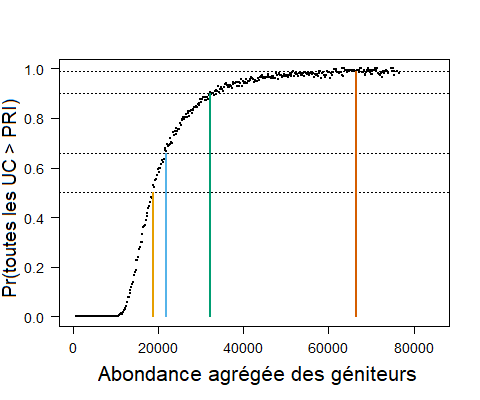
\includegraphics[width=0.6\linewidth]{figure/methods-Example-ProjectedLRP} 

}

\caption{Example of projected probability curve derived from projections over 30 years and 10,000 MC trials.  The curve shows the projected probability of all CUs being above their lower benchmark (LBM) as a function of aggregate SMU abundance, where aggregate spawning abundance is a bin of 200 fish (e.g., 0-200, 201-400, etc.). Each dot in the curve therefore represents a single 200-fish bin. Coloured lines demonstrate how aggregate abundance LRPs are calculated for 4 different probability thresholds: p* = 0.5 (yellow), 0.66 (blue), 0.90 (green), and 0.99 (orange) for the probability that all CUs are greater than their LBM. Horizontal dotted lines intersect the y-axis at each probability threshold, while the solid vertical lines show the corresponding aggregate escapement that will represent the LRP.}\label{fig:example-projectedCurve}
\end{figure}

\end{document}
